\chapter {Manual de GENARO}
\section{Introducci\'on}
\subsection{?`Qu\'e es GENARO?}

GENARO es una herramienta de ayuda a la composici\'on, una opci\'on a la que recurrir si se quiere buscar ideas nuevas. Para tal fin, GENARO compone, mediante ciertos par\'ametros especificados por el usuario, una pieza sencilla. Como esto es un proceso bastante r\'apido, el usuario puede en un peque\~no espacio de tiempo disponer de varias ideas para poder buscar en ellas alguna inspiraci\'on.

\subsection{Historia de GENARO}

GENARO es un programa creado por Javier G\'omez Santos, Juan Rodr\'\i guez Hortal\'a y Roberto Torres de Alba, estudiantes de Ingenier\'\i a Inform\'atica de la Universidad Complutense de Madrid. Surgi\'o como un proyecto para la universidad, en el que no se ten\'\i a muy claro hasta donde podr\'\i a llegarse. Algunos de las propuestas iniciales no pudieron ser alcanzadas, pero muchas de ellas si. Ahora GENARO es un software gratuito para ser usado por cualquiera que quiera buscar ayuda a la composici\'on, o que le apetezca sencillamente jugar un poco con el programa.

\subsection{?`Qu'e es lo que hace GENARO?}
GENARO compone fragmentos musicales para los distintos tipos de pista bas'andose en los fragmentos anteriormente compuestos para otras pistas. De esta manera los fragmentos musicales que suenan a la vez est'an relacionados y `suenan bien` al reproducirse simult'aneamente. En la versi'on actual de GENARO hay dos maneras de generar m'usica:
\begin{enumerate}
\item El acompa~namiento manda: se genera primero el acompa~namiento y a partir de 'el se genera la melod'ia y el bajo.
\item Armonizador: a partir de una melod'ia se genera un acompa~namiento a partir del cu'al se puede generar el bajo.
\end{enumerate}

GENARO permite introducir en sus proyectos cualquier n'umero de pistas de un tipo a elegir entre los tres desarrollados (acompa~namiento, bajo y melod'ia), pudiendo tener cualquier n'umero de pistas del mismo tipo. Las pistas se corresponden con instrumentos que pertenecen a uno de los tres tipos desarrollados.

El producto 'ultimo que nos proporciona GENARO son archivos midi o wav:
\begin{itemize}
\item Midi: es un est'andar en la codificaci'on de partituras por ordenador, permitiendo por tanto al usuario editar y manipular la m'usica compuesta por GENARO con cualquiera de los secuenciadores y programas de edici'on del mercado. Representa la m'usica compuesta como partitura, sin fijar del todo los instrumentos sint'eticos que interpretaran cada pista. Dichos instrumentos se fijar'an definitivamente en el programa que haga de sintetizador del fichero.
\item Wav: es un est'andar en codificaci'on de audio. GENARO tiene incorporado un sintetizador software, Timidity++ (vease secci\'on \ref{timidity} de la p\'agina \pageref{timidity}), que puede realizar el paso a wav del midi generado, asociando a cada pista una fuente de sonido seleccionado de una extensa lista.
\end{itemize}

Debido a las m'ultiples pistas y a la posibilidad de asignar fuentes de sonidos de muchos tipos a cada pista, GENARO es capaz de generar m'usicas muy diversas. En su forma de uso m'as b'asica se puede generar un acompa~namiento de piano y una melodia de piano con un bajo ac'ustico de fondo. Pero pensando un poco surgen m'as opciones, por ejemplo se puede a~nadir otra pista de acompa~namiento que doble a la anterior pero con una fuente de sonido que sean una secci'on de cuerda; o a\~nadir m'as pistas de melod'ia que se contrapongan a la primera, usando fuentes de sonido distintas; o silenciar todo menos el bajo y a\~nadir m'as pistas de bajo, con lo que se obtiene una polifon\'\i a al estilo barroco; o introducir otra pista de acompa\~namiento de piano pero con otro ritmo, para obtener ritmos compuestos...


\subsection{?`C\'omo funciona?}

GENARO ha sido elaborado en tres lenguajes distintos, Prolog, Haskell y C++. En los m\'odulos desarrollados en prolog y haskell es donde residen los algoritmos de inteligencia artificial, que son el n\'ucleo de GENARO, donde se desarrolla la generaci\'on de m\'usica. C++ por su parte se encarga de crear un interfaz gr\'afico agradable para el usuario, y act\'ua como nexo entre los dem\'as lenguajes.

\section {Instalaci\'on}

GENARO no dispone actualmente de instalador, si te has descargado GENARO de internet, lo m\'as probable es que est\'e comprimido en un fichero zip o similar. Tan s\'olo descompr\'\i melo al directorio que desees, y ejecuta el programa \emph{InterfazGenaro.exe} que se halla en el subdirectorio \emph{Codigo/C}.

\section {Manejando a GENARO}

\subsection {Arrancando el programa}

GENARO posee varios ejecutables, pero son casi todos auxiliares, y no deber\'\i an usarse si no se posee un conocimiento claro de como van a reaccionar. Es aconsejable pues ejecutar el programa principal, de nombre \emph{InterfazGenaro.exe}, que se halla en el subdirectorio \emph{Codigo/C}. Este programa se encarga de unir a todos los restantes mediante llamadas totalmente transparentes para el usuario. Una llamada al programa desde otro directorio al suyo, podr�a causar problemas para conseguir encontrar los dem\'as programas y archivos necesarios. Una vez arrancado el interfaz principal, una nueva ventana deber\'\i a aparecer, similar a la mostrada en la figura \ref{InterfazVacio} de la p\'agina \pageref{InterfazVacio}, que ha sido modificada con el fin de hacerla m\'as f\'acil de ver.

\begin{figure}
\centering
    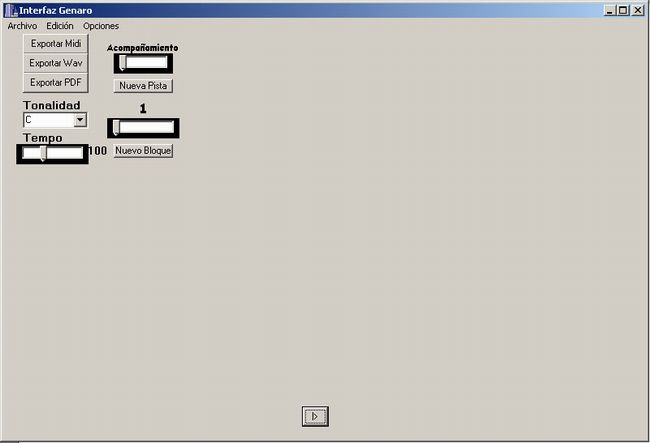
\includegraphics[width=1.0\textwidth]{arrancado1.jpg}
    \caption{Interfaz vac\'\i o tras arrancar}
    \label{InterfazVacio}
\end{figure}

\subsection {Creando un nuevo proyecto}

Una vez hemos arrancado el programa, hemos de crear un nuevo proyecto. Para ello debemos dirigirnos al men\'u \emph{Archivo}, y escoger la opci\'on \emph{Nuevo}, tal y como se muestra en la figura \ref{NuevoProyecto} de la p\'agina \pageref{NuevoProyecto}. Tras esto nos deber\'\i a quedar algo parecido a lo mostrado en la figura \ref{InterfazInicializado} de la p\'agina \pageref{InterfazInicializado}.

\begin{figure}
\centering
    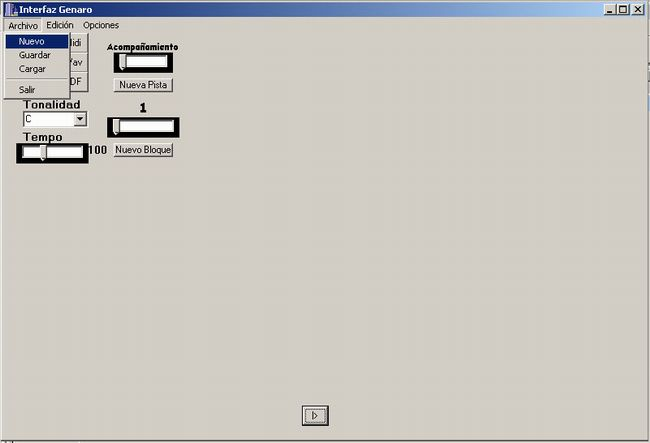
\includegraphics[width=1.0\textwidth]{archivo_nuevo.jpg}
    \caption{Creando un nuevo proyecto}
    \label{NuevoProyecto}
\end{figure}

\begin{figure}
\centering
    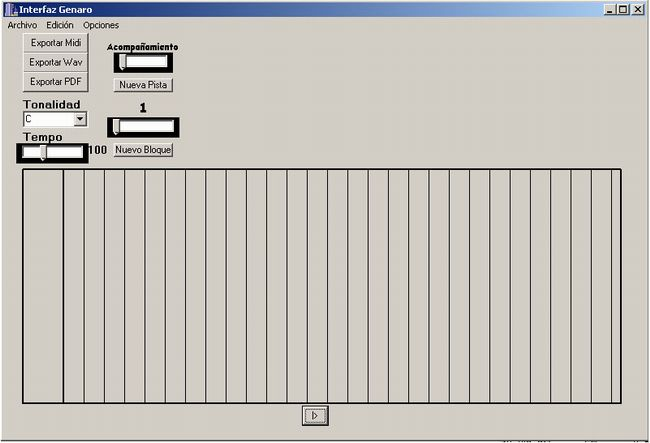
\includegraphics[width=1.0\textwidth]{ya_Inicializado.jpg}
    \caption{Interfaz tras pulsar el bot\'on \emph{nuevo}}
    \label{InterfazInicializado}
\end{figure}

\subsection {Creando pistas}

Un proyecto GENARO consta de un n\'umero variable de pistas. Una pista es un conjunto de sonidos asignados a un instrumento. Para GENARO existen 3 tipos distintos de pistas, la pista de \emph{acompa\~namiento}, la pista de \emph{melod\'\i}a y la pista de \emph{bajo}. Cada una de estas pistas funciona de manera distinta, y puede haber cualquier n\'umero de ellas, a excepci\'on de la pista de acompa\~namiento, ya que ha de haber siempre un m\'\i nimo de 1.\\
Para crear una nueva pista, debemos mover el selector que se encuentra situado encima del bot\'on \emph{Nueva Pista}, arriba a la izquierda. Al desplazarlo vemos como cambia el tipo de pista seleccionado, mostrando cualquiera de los anteriormente mencionados. Cuando hayamos encontrado el que buscamos, pulsamos el bot\'on \emph{Nueva Pista}. Una nueva divisi\'on vertical debe haber aparecido, con un cuadro coloreado a la izquierda. Esto es una pista. En la figura \ref{InterfazPistasCreadas} de la p\'agina \pageref{InterfazPistasCreadas} vemos un ejemplo con 5 pistas creadas. Los colores nos ayudan a distinguir el tipo de pista, as\'\i ~las pistas \emph{blancas} corresponden a \emph{acompa\~namiento}, las \emph{verdes} son las pistas de \emph{Melod\'\i a}, y las \emph{azules} las de \emph{bajo}.

\begin{figure}
\centering
    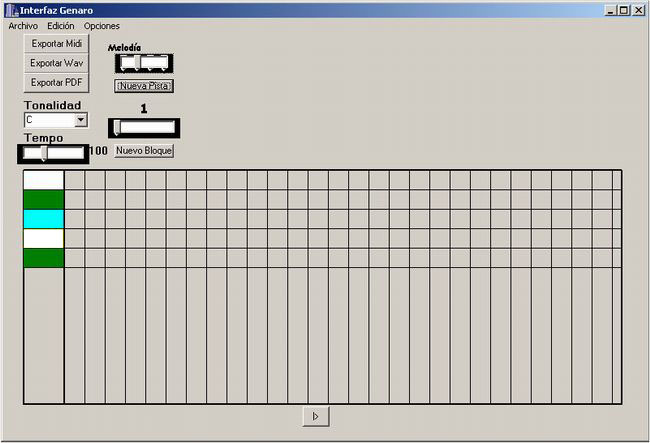
\includegraphics[width=1.0\textwidth]{Pistas_Creadas.jpg}
    \caption{Creando varias pistas}
    \label{InterfazPistasCreadas}
\end{figure}

\subsection {Creando bloques}

Para GENARO, una divisi\'on horizontal o en el tiempo es un \emph{bloque}. Un conjunto de sonidos que tienen sentido musical por si mismos. El usuario puede decidir crear 1 o varios bloques para una pieza GENARO, que en su conjunto formar\'an la pieza que compondr\'a GENARO. Para crear un nuevo bloque en el proyecto, has de elegir primero el n\'umero de compases que quieres para ese bloque, mediante el selector que hay sobre el bot\'on \emph{Crear Bloque}, y despu\'es has de pinchar sobre el bot\'on \emph{Crear Bloque}. Un ejemplo con un bloque ya creado lo podemos ver en la figura \ref{InterfazBloqueCreado} de la p�gina \pageref{InterfazBloqueCreado}. El color del bloque es rojo si este no ha sido inicializado, o el usuario ha decidido silenciarlo.

\begin{figure}
\centering
    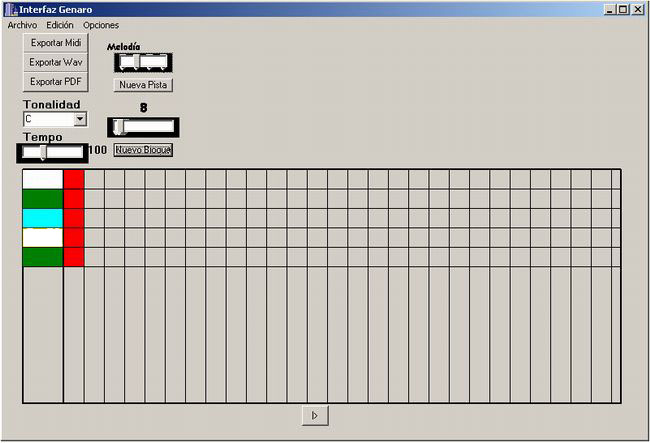
\includegraphics[width=1.0\textwidth]{Bloque_Creado.jpg}
    \caption{Ejemplo de proyecto con un bloque creado}
    \label{InterfazBloqueCreado}
\end{figure}

\subsection {Editando la cabecera de una pista}

Como ya dijimos antes, una pista es un conjunto de sonidos asignados a un instrumento. Una pista esta formada por varios sub-bloques, que son la intersecci\'on entre una pista y un bloque. Podemos cambiar algunas opciones generales de una pista si pinchamos con el rat\'on sobre su cabecera, que corresponde al primer recuadro de la pista. Tras pinchar en este recuadro aparecer\'a ante nosotros un nuevo cuadro de opciones, situado arriba a la derecha, como se muestra en la figura \ref{InterfazEditandoPista} de la p\'agina \pageref{InterfazEditandoPista}.\\
En este nuevo cuadro podemos distinguir varios elementos:
\begin {enumerate}
\item Una etiqueta que nos recuerda que pista estamos modificando (en este caso la \emph{pista 0}).
\item Una etiqueta que nos recuerda que tipo de pista estamos modificando (en este caso una pista de \emph{Acompa\~namiento}).
\item Una opci\'on para silenciar toda la pista, de tal manera que la pieza creada prescindir\'\i a de reproducir esta pista.
\item Una lista de instrumentos midi, para poder elegir con cual interpretar la pista.
\item Un bot\'on \emph{Guardar} para guardar los cambios realizados en la pista.
\end {enumerate}.

\begin{figure}
\centering
    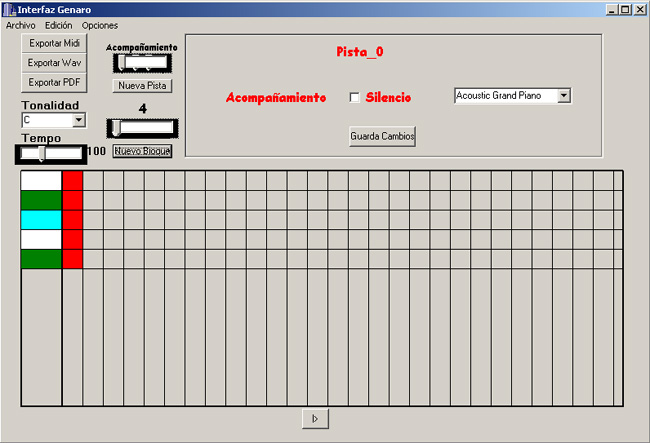
\includegraphics[width=1.0\textwidth]{Edicion_Pista.jpg}
    \caption{Editando las opciones de una pista}
    \label{InterfazEditandoPista}
\end{figure}

\subsection{Editando un sub-bloque de una pista}

Para editar un sub-bloque de un pista, debemos pinchar sobre el sub-bloque correspondiente. Dependiendo del tipo de pista en la que estemos editando el sub-bloque podremos dar unos par\'ametros u otros, pero todos los sub-bloques tienen unas opciones en com\'un, las \emph{Opciones Generales}, que son las que aparecen en la figura \ref{InterfazBloqueGeneral} de la p\'agina \pageref{InterfazBloqueGeneral}.

\begin{figure}
\centering
    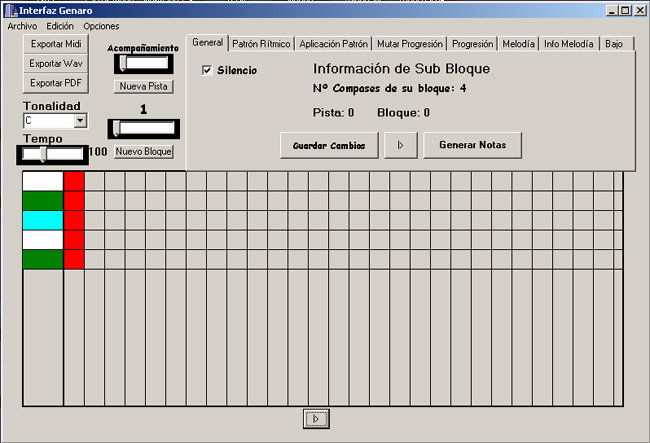
\includegraphics[width=1.0\textwidth]{General_Bloque.jpg}
    \caption{Editando las opciones generales de un sub-bloque}
    \label{InterfazBloqueGeneral}
\end{figure}

En este recuadro de opciones generales podemos distinguir varias partes:
\begin {enumerate}
\item Una etiqueta que nos recuerda el n\'umero de compases del bloque al que pertenece.
\item Dos etiquetas que nos informan de a que pista y a que bloque pertenece el sub-bloque que estamos editando.
\item Una opci\'on para silenciar el sub-bloque, y no ser interpretado en la pieza.
\item Un bot\'on para guardar los cambios realizados en el sub-bloque
\item Un bot\'on para generar el fragmento musical correspondiente a este sub-bloque, que es obligatorio generar antes de componer la pieza final. Dependiendo del tipo de pista en la que nos encontremos, tendremos que haber dado algunos par\'ametros u otros al programa.
\item Un bot\'on para reproducir el fragmento musical perteneciente a este sub-bloque.
\end{enumerate}

A continuaci\'on veremos las opciones de cada tipo de pista.

\subsubsection{Editando un sub-bloque de acompa\~namiento}

Un sub-bloque de acompa\~namiento ha de tener asignado una progresi\'on para poder generar su parte correspondiendte. Tambi\'en es aconsejable haber modificado los par\'ametros que vienen por defecto. Los par\'ametros que se deben modificar est\'an agrupados en 2 tipos, los par\'ametros correspondientes al \emph{Patr\'on R\'\i tmico} y a su aplicaci\'on, y a los correspondientes a la \emph{progresi\'on}.

\begin {enumerate}
\item Si vamos a modificar los par\'ametros correspondientes al \emph{Patr\'on R\'\i tmico}, tendremos ante nosotros una imagen como la mostrada en la figura \ref{InterfazBloquePatron} de la p\'agina \pageref{InterfazBloquePatron}. Los par\'ametros que se pueden modificar en este cuadro son:

\begin{figure}
\centering
    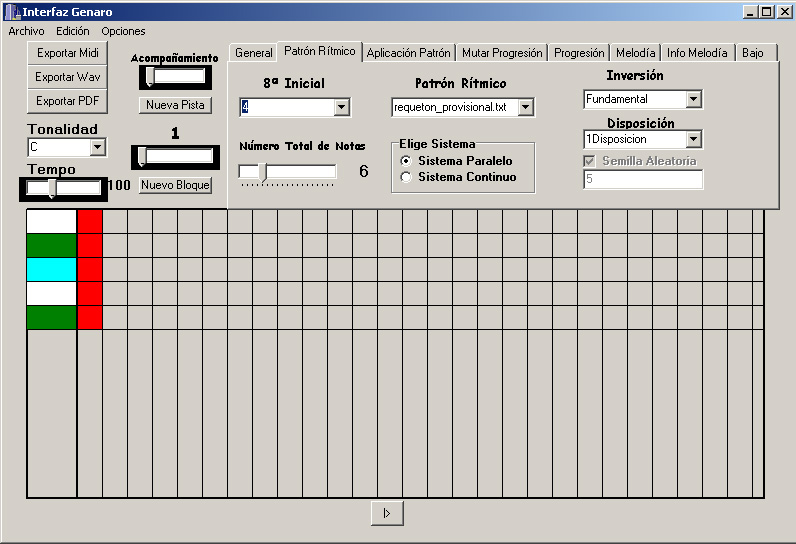
\includegraphics[width=1.0\textwidth]{bloque_acomp_patron.jpg}
    \caption{Editando las opciones de patr\'on r\'\i tmico de un sub-bloque}
    \label{InterfazBloquePatron}
\end{figure}

\begin {itemize}
\item [Patr\'on R\'\i tmico:] es una lista desplegable que te permite elegir entre los patrones disponibles, algunos se distribuyen con GENARO, mientras que otros los puedes crear t\'u mismo usando el \emph{Editor de Pianola} que viene con GENARO. Para m\'as informaci\'on sobre el editor de pianola, o de como modificar un patr\'on r\'\i tmico existente, consulta la secci\'on dedicada al editor de pianola, secci\'on \ref{edipianola} de la p\'agina{edipianola}.
\item [$8^{a}$ Inicial:] consiste en una lista desplegable que nos permite elegir entre un n�mero comprendido entre 1 y 7. La octava aconsejable es la 4, con una octava m\'as baja obtendr\'as un sonido m\'as grave, mientras que si escoges una octava mayor, el sonido ser\'a m\'as agudo.
\item [N\'umero total de notas:] es el n\'umero de notas que pueden sonar simult\'aneamente en la pieza, es aconsejable usar un valor pr\'oximo a 6.
\item [Sistema:] Existen 2 sistemas para generar el fragmento, cada uno de ellos tiene sus opciones independientes. Estos sistemas son el \emph{sistema paralelo}, que te pide que elijas \emph{Inversi\'on} y \emph{Disposici\'on}, mientras que el \emph{sistema continuo} te permite especificar una semilla en lugar de generarla aleatoriamente.
\end {itemize}

\item Para modificar los par\'ametros correspondientes a la aplicaci\'on del patr\'on, nos encontraremos ante un cuadro de opcioens como el mostrado en la figura \ref{InterfazBloqueAplicPatron} de la p\'agina \pageref{InterfazBloqueAplicPatron}. Aqu\'\i ~podemos modificar los siguientes par\'ametros:

\begin{figure}
\centering
    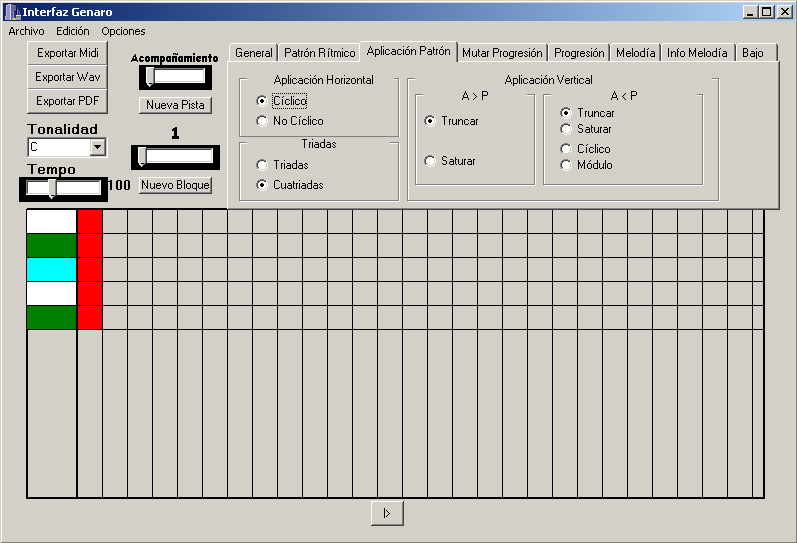
\includegraphics[width=1.0\textwidth]{bloque_acomp_aplic_patron.jpg}
    \caption{Editando las opciones de aplicaci\'on del patr\'on r\'\i tmico de un sub-bloque}
    \label{InterfazBloqueAplicPatron}
\end{figure}

\begin {itemize}
\item [Aplicaci\'on Horizontal:] podemos elegir entre realizar la aplicaci\'on horizontal del patr\'on de manera \emph {C\'\i clica} o \emph {No c\'\i clica}.
\item [Aplicaci\'on Vertical:] aqu\'\i ~debemos especificar que acciones tomar\'a para 2 casos, cuando hay mas acordes que patrones, en cuyo caso tendremos que especificar si queremos \emph{truncar} o \emph{saturar}, y el caso opuesto, donde tendremos que especificar si queremos \emph{truncar}, \emph{saturar}, \emph{c\'\i clico} o \emph{m\'odulo}.
\item [Triadas:] tendremos que especificar si preferimos \emph{triadas} o \emph{cuatriadas}.
\end {itemize}

\item Antes de crear una progresi\'on tenemos que especificar el n\'umero de mutaciones que queremos, para ello vamos al cuadro \emph{Mutar Progresi\'on}. Existen 5 tipos distintos de mutaciones, \emph{Juntar Acordes}, \emph{Separar Acordes}, \emph{Cambiar Acordes}, \emph{Dominantes Secundario} y \emph{Segunda Menor S\'eptima}. Estas mutaciones est\'an a su vez agrupadas en 2 grandes tipos, as\'\i ~pues las 3 primeras pertenecen al \emph{Tipo A}, y las 2 \'ultimas al \emph{Tipo B}. El usuario puede elegir entre realizar un n\'umero de mutaciones independientemente del tipo, (opci\'on \emph{Mutaciones Totales}), o bien especificar cuantas mutaciones de cada tipo prefiere, mediante las barras de desplazamiento que se muestran en la figura \ref{InterfazBloqueMutaProg} de la p\'agina \pageref{InterfazBloqueMutaProg}.

\begin{figure}
\centering
    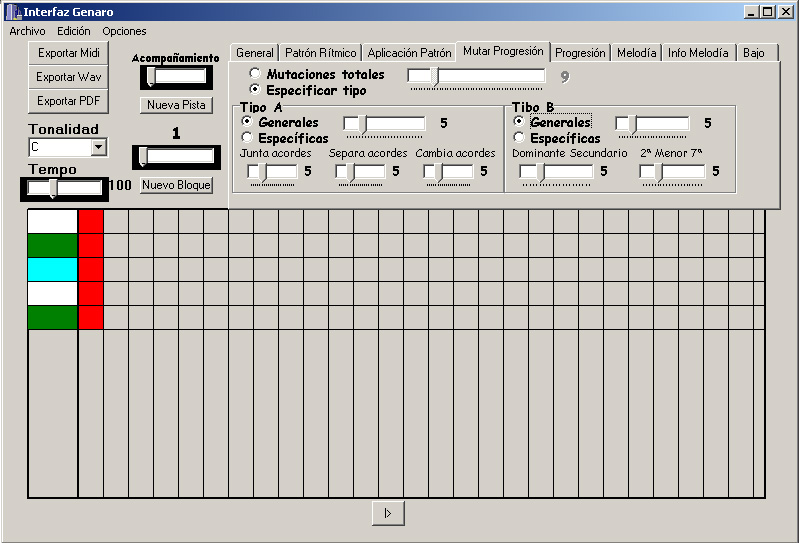
\includegraphics[width=1.0\textwidth]{bloque_acomp_mutap.jpg}
    \caption{Editando las opciones de mutaci\'on de una progresi\'on}
    \label{InterfazBloqueMutaProg}
\end{figure}

\item Para crear una progresi\'on, o usar una ya creada, tenemos que irnos al cuadro \emph{Progresi\'on}, tras esto tendremos una imagen similar a la que aparece en la figura \ref{InterfazBloqueProg} de la p\'agina \pageref{InterfazBloqueProg}. En este cuadro encontraremos las siguientes opciones:

\begin{figure}
\centering
    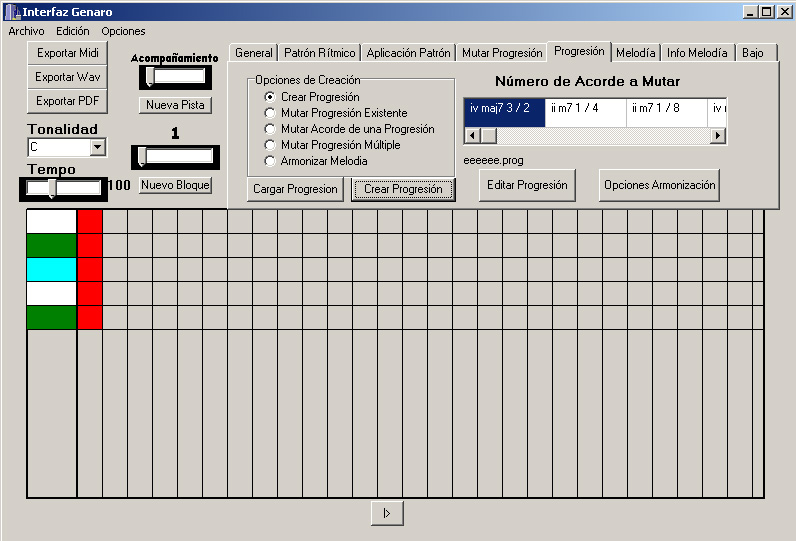
\includegraphics[width=1.0\textwidth]{bloque_acomp_prog.jpg}
    \caption{Editando las opciones de creaci\'on de una progresi\'on}
    \label{InterfazBloqueProg}
\end{figure}

\begin {itemize}
\item \emph{Opciones de Creaci\'on:} nos permite elegir entre las distintas formas de crear una progresi\'on. las analizaremos mas adelante en profundidad.
\item \emph{Cargar Progresi\'on:} si preferimos usar una progresi\'on creada anteriormente, tendremos que pulsar este bot\'on, y especificar cual es la progresi\'on que queremos usar.
\item \emph{Crear Progresi\'on:} tras escoger la opci\'on de creaci\'on, si pulsamos este bot\'on crearemos una nueva progresi\'on con el nombre que especifiquemos.
\item \emph{Progresi\'on:} En un grid aparecer\'a la progresi\'on con la que estemos trabajando actualmente, con su nombre debajo. Hay que tener en cuenta que el acorde que tenemos seleccionado ser\'a el acorde en el que realizaremos la mutaci\'on en caso de escoger la opci\'on \emph{Mutar acorde de una progresi\'on}.
\item \emph{Editar Progresi\'on:} si pulsamos este bot\'on abriremos una nueva ventana para editar la progresi\'on con la que estamos trabajando. La ventana que aparece se muestra en la figura \ref{InterfazEditaProg} de la p\'agina \pageref{InterfazEditaProg}. Nos permite crear nuevos acordes y sustituir los existentes, o a\~nadirlos delante o detras de los mismos. 
\item \emph{Opciones de Armonizaci\'on:} Al igual que en el caso anterior, este bot\'on crear\'a una nueva ventana que nos permitir\'a elegir entre distintas opciones de armonizaci\'on, tal y como se muestra en la figura \ref{InterfazEditaArmon} de la p\'agina \pageref{InterfazEditaArmon}.
\end {itemize} 

\begin{figure}
\centering
    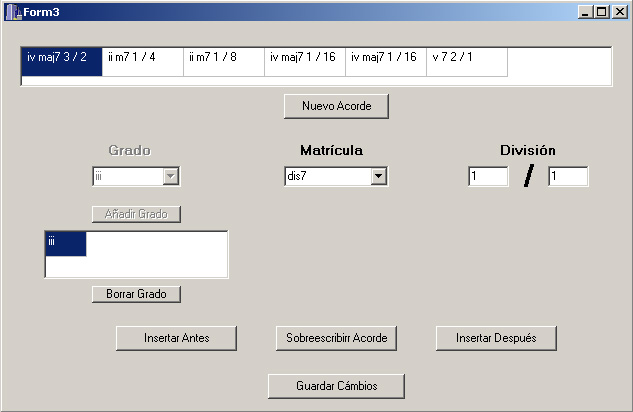
\includegraphics[width=1.0\textwidth]{Editar_Progresion.jpg}
    \caption{Editando una progresi\'on}
    \label{InterfazEditaProg}
\end{figure}

\begin{figure}
\centering
    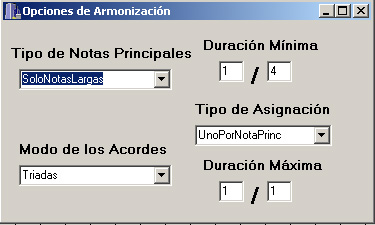
\includegraphics[width=0.7\textwidth]{opciones_armon.jpg}
    \caption{Opciones de armonizacion}
    \label{InterfazEditaArmon}
\end{figure}

Con respecto a las opciones de creaci\'on de progresi\'on, podemos distinguir las siguientes:
\begin {itemize}
\item \emph{Crear Progresi\'on:} crea una nueva progresi\'on con los par\'ametros de mutaci\'on anteriormente especificados
\item \emph{Mutar Progresi\'on Existente:} genera una nueva progresi\'on a partir de una progresi'on ya dada, aplicando las mutaciones especificadas anteriormente.
\item \emph{Mutar Acorde de una Progresi\'on:} muta el acorde seleccionado en la progresi\'on aplicando las mutaciones especificadas.
\item \emph{Mutar Progresi\'on M\'ultiple:} permite crear una progresi\'on tomando la semilla de una progresi\'on ya existente
\item \emph{Armonizar Melod\'\i a:} Permite coger una pista de melod\'\i a para crear una progresi\'on con ella.
\end {itemize}

No debemos olvidar que una vez hayamos terminado de especificar todas las opciones necesarias, tenemos que ir a las opciones generales y generar las notas correspondientes al sub-bloque actual (para ello pulsa el bot\'on \emph{Generar Notas}). Un sub-bloque que no est\'a silenciado se dibuja de color \emph{azul}, en vez del color \emph{rojo} con el que aparece inicialmente.

\end {enumerate}

\subsubsection{Editando un sub-bloque de melod\'\i a}

Una melod\'\i a precisa de una pista de acompa\~namiento para poder componer su fragmento. Es necesario que al menos hayas creado la progresi\'on de la pista de acompa\~namiento que va a tomar como referencia la melod\'\i a para poder componer su fragmento. Los distintos cuadros que nos permiten alterar los par\'ametros de creaci\'on de una melod\'\i a son los siguientes:

\begin {enumerate}
\item los par\'ametros que se hallan en el cuadro \emph{Melod\'\i a} (mostrado en la figura \ref{EditaBloqueMelodica} de la p\'agina \pageref{EditaBloqueMelodica}) van a determinar la melod\'\i a que se va a generar. Los par\'ametros que aqu\'\i ~se encuentran son:

\begin{figure}
\centering
    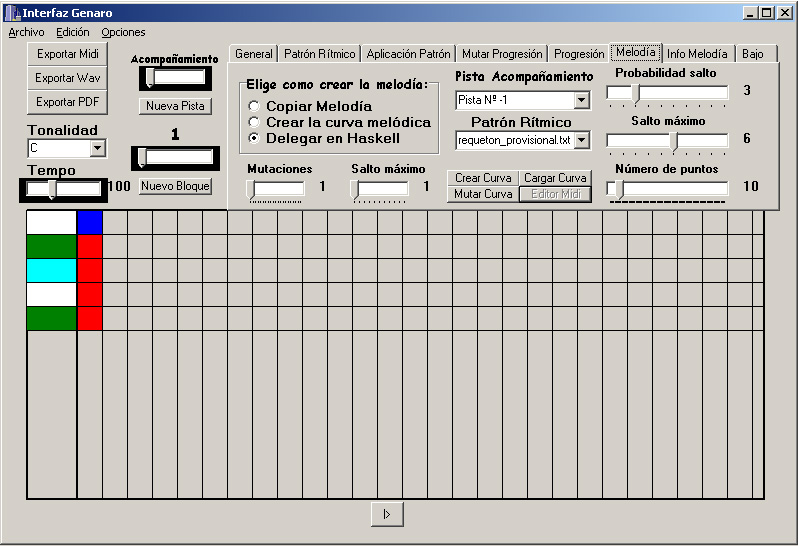
\includegraphics[width=1.0\textwidth]{Bloque_Melodia.jpg}
    \caption{Editando una melod\'\i a}
    \label{EditaBloqueMelodica}
\end{figure}

\begin {itemize}
\item \emph{Elige como crear la melod\'\i a:} que tiene tres opciones, \emph{Copiar Melod\'\i a} de otro sub-bloque de melod\'\i a, creando una curva mel\'odica o delegando en haskell para que cree una curva mel\'odica.
\item \emph{Pista de Acompa\~namiento:} en esta lista tenemos todas las pistas de acompa\~namiento existentes, tenemos que seleccionar una.
\item \emph{atr\'on R\'\i tmico:} una lista con los patrones existentes, para tomar como base para crear la melod\'\i a.
\item \emph{Bot\'on Crea Curva:} que dependiendo de la opci\'on marcada en \emph{Elige como crear la melod\'\i a} usar\'a los par\'ametros establecidos a su derecha para llamar a haskell y crear una nueva curva, o bien arrancar\'a una nueva ventana como la mostrada en la figura \ref{EditaCurvaMelodica} de la p\'agina \pageref{EditaCurvaMelodica} para que el usuario pueda crear o editar la suya propia.
\item \emph{Bot\'on Cargar Curva:} si tenemos intenci\'on de usar alguna curva ya creada anteriormente. Hay que tener en mente que las curvas se crean con nombres autom\'aticos, con 2 n\'umeros que corresponden a la pista y al bloque.
\item \emph{Bot\'on Mutar Curva:} para mutar la curva existente, usando los par\'ametros que hay a la izquierda de este bot\'on.
\end {itemize}

\begin{figure}
\centering
    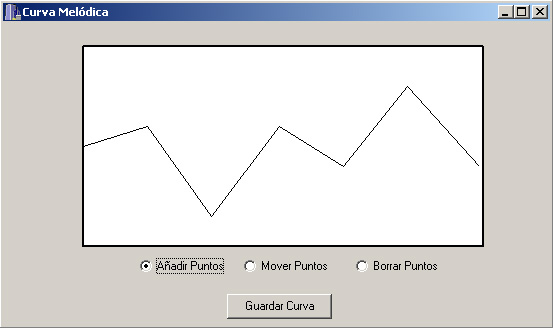
\includegraphics[width=0.7\textwidth]{curva_mel.jpg}
    \caption{Editando una curva mel\'odica}
    \label{EditaCurvaMelodica}
\end{figure}

\item Otras opciones que podemos especificar para crear la melod\'\i a est\'an en el cuadro \emph{Info Melod\'\i a}, como se muestra en la figura \ref{EditaInfoMelodica} de la p\'agina \pageref{EditaInfoMelodica}, pueden ser tambi\'en alteradas, para producir un resultado distinto, estas opciones son 4 barras de desplazamiento que nos permiten elegir entre \emph{velocidad de trino}, \emph{Dividir notas}, \emph{Alargar notas} y \emph{Trinos}.

\begin{figure}
\centering
    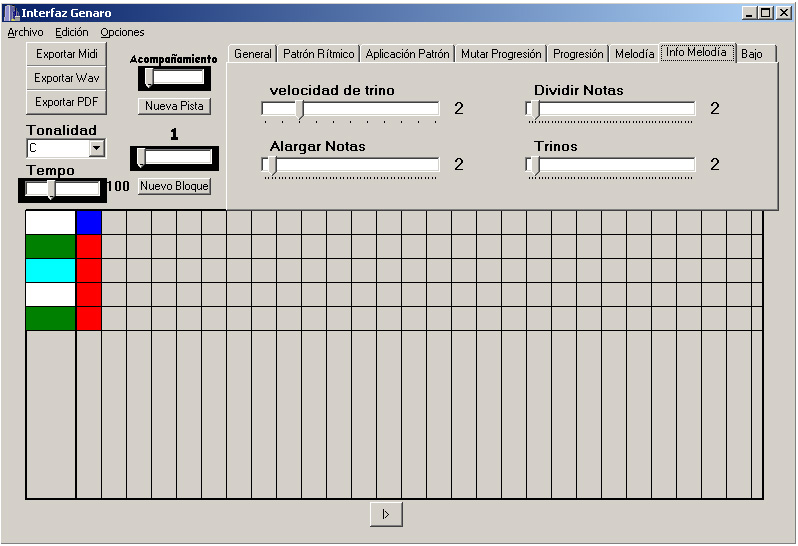
\includegraphics[width=1.0\textwidth]{Bloque_Melodia2.jpg}
    \caption{Editando una melod\'\i a, parte 2}
    \label{EditaInfoMelodica}
\end{figure}
 
\end {enumerate}

\subsubsection{Editando un sub-bloque de Bajo}

El bloque de \emph{Bajo} tiene s\'olo un cuadro para cambiar par\'ametros, es el mostrado en la figura \ref{EditaBloqueBajo} de la p\'agina \pageref{EditaBloqueBajo}. Los m\'as relevantes son:

\begin{figure}
\centering
    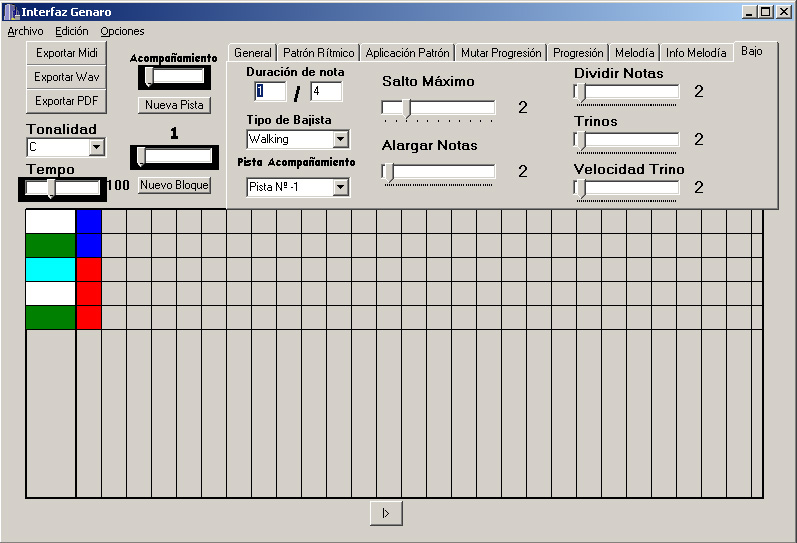
\includegraphics[width=1.0\textwidth]{bloque_bajo.jpg}
    \caption{Editando una sub-bloque de Bajo}
    \label{EditaBloqueBajo}
\end{figure}

\begin {itemize}
\item \emph{Pista de Acompa\~namiento:} en esta lista tenemos todas las pistas de acompa\~namiento existentes, tenemos que seleccionar una.
\item \emph{Tipo de bajista:} una lista de 3 bajistas, cada uno compone de una manera muy distinta al otro.
\item \emph{Duraci\'on de la nota:} que es una fracci\'on de n\'umeros naturales
\item \emph{Otros Par\'ametros:} sin ser tan importante como estos, existen otros 5 par\'ametros que nos permiten configurara a nuestro gusto el bajo, son \emph{Salto M\'aximo}, \emph{velocidad de trino}, \emph{Dividir notas}, \emph{Alargar notas} y \emph{Trinos}.

\end {itemize}

\subsection{Creando la pieza final}

Si ya has terminado de inicializar todos los sub-bloques correspondientes a tu proyecto, tan s\'olo queda crear el midi final. Antes de esto tienes que especificar la \emph{tonalidad} con la que quieres crear tu pieza, (viene en notaci\'on americana), est\'a en la lista que hay a la izquierda del todo, y justo debajo hay un selector para ponerle el \emph{Tempo} que quieras a tu obra. Si est\'as de acuerdo con la tonalidad y tempo que has elegido, presiona el bot\'on \emph{Exportar Midi}, y tras unos segundos tu midi estar\'a creado. Se halla en el directorio ra\'\i z del programa, con el nombre de \emph{musica-genara.mid}, pero te aconsejamos que lo reproduzcas dir\'ectamente desde el interfaz, ya que est\'a enlazado con \emph{Timidity}, un excelente programa de reproducci\'on de midis, con el que escuchar\'as tu pieza con gran calidad. Existen tambi\'en opciones de reproducci\'on en genaro, pero las vamos a especificamos en la secci\'on \ref{oprepro} de la p\'agina \pageref{oprepro}.

\subsection{Opciones de reproducci\'on}
\label{oprepro}
El usuario puede editar las opciones de reproducci\'on de midi del programa \emph{Timidity} pulsando sobre el men\'u \emph{Opciones} y posteriormente pulsando en \emph{Reproducci\'on}. Tras esto aparecer\'a una nueva ventana como la mostrada en la figura \ref{OpcionesRepro} de la p\'agina \pageref{OpcionesRepro}. Esta nueva ventana te permite modificar los siguientes par\'ametros de reproducci\'on:

\begin{figure}
\centering
    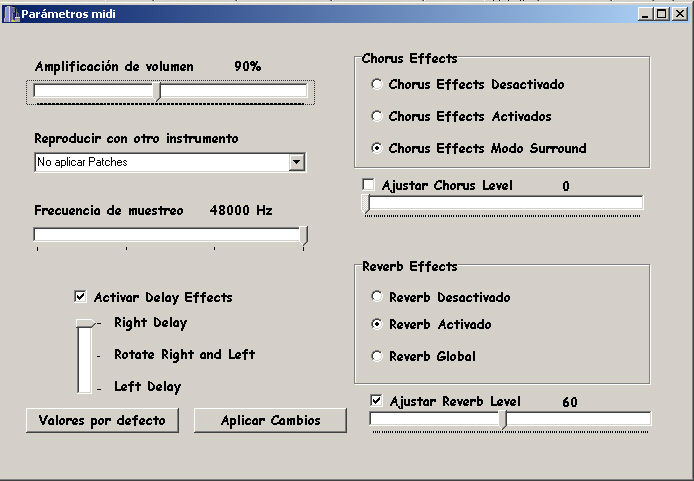
\includegraphics[width=1.0\textwidth]{param_repro.jpg}
    \caption{Opciones de reproducci\'on para el midi}
    \label{OpcionesRepro}
\end{figure}

\begin {itemize}
\item \emph{Amplificaci\'on de volumen:} permite modificar el volumen con el que \emph{Timidity} va a reproducir/exportar la pieza.
\item \emph{Chorus Effects:} permite activar/desactivar los coros, eligiendo el modo. Tambi\'en se puede especificar el level mediante la barra de desplazamiento que hay bajo esta opci\'on.
\item \emph{Reproducir con otro instrumento:} es una lista que permite elegir un \emph{patch} para reproducir todas las pistas con este instrumento.
\item \emph{Frecuencia de muestreo:} te permite cambiar el n\'umero de muestras por segundos
\item \emph{Reverb Effects:} puedes activar y desactivar el efecto reverb, y ajustar el nivel del mismo.
\item \emph{Usar Delay Effects:} para activar el efecto delay, con opciones de usarlo a la izquierda, derecha o rotarlo.
\item \emph{Bot\'on Valores por defecto:} al pulsar este bot\'on pone todos los par\'ametros al valor por defecto.
\item \emph{Bot\'on Aplicar Cambios:} guarda los cambias realizados en las opciones de reproducci\'on. Si no pulsas este bot\'on se descartar\'an los cambios hechos.
\end {itemize}

\subsection{Exportando a wav}

Exportar a wav es una opci\'on que permite una vez generado el archivo midi, crear un archivo wav. Para ello llama a \emph{timidity} con los par\'ametros de reproducci\'on especificados por el usuario en \emph{Opciones de Reproducci\'on}, y crea un fichero wav con el nombre de \emph{musica-genara.wav}, que se encuentra en el directorio ra\'\i z del programa. Para exportar el fichero midi a wav, tan s\'olo pulsa sobre el bot\'on \emph{Exportar a Wav} que se encuentra debajo del bot\'on \emph{Exportar a Midi}.

\subsection{Guardando y cargando proyectos}

GENARO permite guardar un proyecto para poder trabajar con el posteriormente. Para ello dir\'\i gete al men\'u \emph{Archivo} y escoge la opci\'on \emph{Guardar}. El programa te preguntar\'a por el nombre con el que quieres guardar el proyecto, y posteriormente lo guardar\'a con el nombre proporcionado.\\
Para cargar un archivo, dir\'\i gete al men\'u \emph{Archivo}, y escoge la opci\'on \emph{Cargar}. Escoge el archivo de proyecto que desees, y contin\'ua trabajando donde lo dejastes.

\section{El editor de pianola}
\label{edipianola}
El editor de pianola es una utilidad que acompa\~na a GENARO para la edici\'on y creaci\'on de patrones r\'\i tmicos. Un patr\'on r\'\i tmico es una estructura capaz de organizar las voces de un acorde en el tiempo. Es un componente no aleatorio.\\
Para ejecutar el editor de pianola, has de pulsar sobre el men\'u \emph{Edici\'on} del programa principal, escoger la opci\'on \emph{Editor de pianola}, y te aparecer\'a una nueva ventana como la mostrada en la figura \ref{EditorPianola} de la p\'agina \pageref{EditorPianola}.

\begin{figure}
\centering
    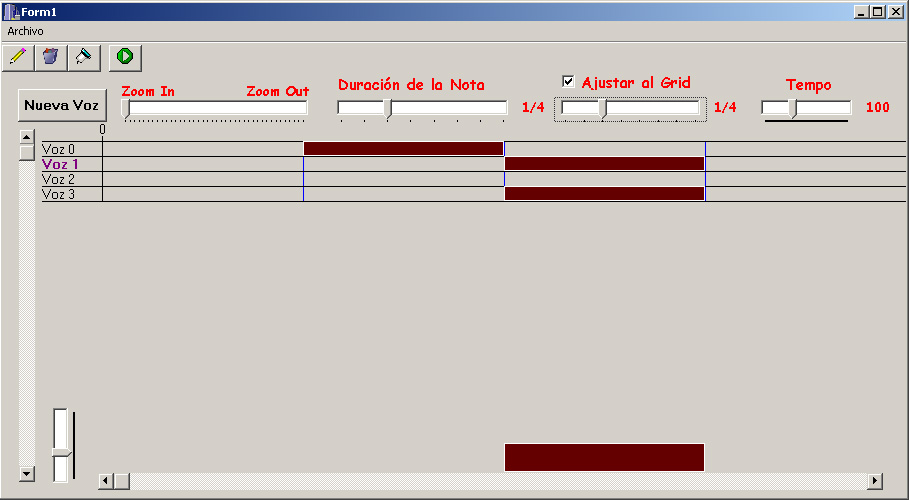
\includegraphics[width=1.0\textwidth]{editorpianola.jpg}
    \caption{El editor de pianola}
    \label{EditorPianola}
\end{figure}

\subsection {Creando un nuevo proyecto}

Al igual que con el programa principal, para trabajar con el editor de pianola tenemos que crear un nuevo proyecto, o bien, cargar uno existente. Para crear un nuevo proyecto, sencillamente dir\'\i gete al men\'u \emph{Archivo}, y escoge la opci\'on \emph{Nuevo}. Tras esto ya puedes empezar a trabajar en el patr\'on r\'\i tmico.

\subsection {Creando voces en el editor de pianola}

Para crear una nueva voz en el editor de pianol, tan s\'olo has de pulsar sobre el bot\'on \emph{Nueva Voz} que se encuentra arriba a la izquierda. Cada vez que pulses este bot\'on, una nueva fila aparecer\'a  en el editor. Si creas m\'as filas de las que es capaz de mostrar el editor, podr\'as desplazarte por ellas mediante el uso de la barra de desplazamiento vertical que hay a la izquierda del todo.

\subsection {Aumentando la resoluci\'on del editor}

Como habr\'as observado, el editor de pianola posee una barra de desplazamiento con las palabras \emph{Zoom In} y \emph{Zoom out}. Al desplazar la barra en un sentido o en otro, aumentamos o disminuimos el tama\~no con el que vemos la rejilla.

\subsection {Eligiendo la duraci\'on de la nota que vamos a a\~nadir}

Cuando estemos en \emph{modo edici\'on}, cada vez que pulsemos sobre la rejilla intentaremos a\~nadir una nueva nota. Esta nota tendr\'a la duraci\'on determinada por la barra de desplazamiento \emph{Duraci\'on de la nota}.

\subsection {El grid, divisiones para facilitar la edici\'on}

El editor de pianola permite crear separaciones de la duraci\'on especificada por el usuario, para hacer mas c\'omoda la edici\'on. Para ello debemos desplazar la barra \emph{Ajustar al Grid}. Posee tambi\'en una opci\'on para ajustar la nota al grid, marcando la casilla que hay en \emph{Ajustar al Grid}. Con esta opci\'on marcada, cualquier nota que se a\~nada al patr\'on, se pondr\'a en la zona a la que pertenezca la divisi\'on especificada en \emph{Ajustar al Grid}.

\subsection {El men\'u edici\'on}

Justo debajo del men\'u del editor de pianola, encontramos 4 botones. Su funci\'on es la siguiente:

\begin{itemize}
\item [L\'apiz:] Es el bot\'on edici\'on, mientras este bot\'on est\'e pulsado, cada vez que pinchemos sobre la rejilla intentaremos insertar una nueva nota
\item [Papelera:] Es el bot\'on eliminar. Nos permite borrar notas de la rejilla pinchando sobre ellas.
\item [Escaner:] Es el bot\'on examinar. Nos permite seleccionar una voz sin realizar ning\'un cambio en el sistema. Tambi\'en nos permite modificar el \emph{Velocity} de cada nota.
\item [Play:] Es el bot\'on reproducir, nos permite escuchar como sonar\'\i a el patr\'on que estamos componiendo. Para cambiar el tempo de esta reproducci\'on debemos mover la barra de desplazamiento llamada \emph{Tempo}
\end{itemize}

\subsection{El velocity}

El velocity corresponde por ejemplo a la \emph{fuerza} con la que se pulsa una tecla en un piano, podemos modificar el velocity de cada nota escogiendo el \emph{modo examinar}, y pinchando sobre la parte inferior de la rejilla, subiendo o bajando el rect\'angulo que aparece, observese que dependiendo de su altura el color de este rect\'angulo y de la nota a la que pertenece cambian.\\
Podemos ajustar un velocity por defecto moviendo el selector que hay debajo de la rejilla.

\subsection {Guardando y cargando}

Si queremos guardar el patr\'on, debemos pulsar sobre el men\'u \emph{Archivo}, y en la opci\'on \emph{Guardar}. El programa nos pedir\'a con que nombre queremos guardar este patr\'on. Es importanto que los patrones se guarden en el subdirectorio del programa \emph{PatronesRitmicos}, ya que ah\'\i ~es donde los busca GENARO.\\
Para cargar un patr\'on debemos dirigirnos al men\'u \emph{Archivo}, y escoger la opci\'on \emph{Cargar}.

